% Options for packages loaded elsewhere
\PassOptionsToPackage{unicode}{hyperref}
\PassOptionsToPackage{hyphens}{url}
%
\documentclass[
]{article}
\usepackage{amsmath,amssymb}
\usepackage{iftex}
\ifPDFTeX
  \usepackage[T1]{fontenc}
  \usepackage[utf8]{inputenc}
  \usepackage{textcomp} % provide euro and other symbols
\else % if luatex or xetex
  \usepackage{unicode-math} % this also loads fontspec
  \defaultfontfeatures{Scale=MatchLowercase}
  \defaultfontfeatures[\rmfamily]{Ligatures=TeX,Scale=1}
\fi
\usepackage{lmodern}
\ifPDFTeX\else
  % xetex/luatex font selection
\fi
% Use upquote if available, for straight quotes in verbatim environments
\IfFileExists{upquote.sty}{\usepackage{upquote}}{}
\IfFileExists{microtype.sty}{% use microtype if available
  \usepackage[]{microtype}
  \UseMicrotypeSet[protrusion]{basicmath} % disable protrusion for tt fonts
}{}
\makeatletter
\@ifundefined{KOMAClassName}{% if non-KOMA class
  \IfFileExists{parskip.sty}{%
    \usepackage{parskip}
  }{% else
    \setlength{\parindent}{0pt}
    \setlength{\parskip}{6pt plus 2pt minus 1pt}}
}{% if KOMA class
  \KOMAoptions{parskip=half}}
\makeatother
\usepackage{xcolor}
\usepackage[margin=1in]{geometry}
\usepackage{graphicx}
\makeatletter
\def\maxwidth{\ifdim\Gin@nat@width>\linewidth\linewidth\else\Gin@nat@width\fi}
\def\maxheight{\ifdim\Gin@nat@height>\textheight\textheight\else\Gin@nat@height\fi}
\makeatother
% Scale images if necessary, so that they will not overflow the page
% margins by default, and it is still possible to overwrite the defaults
% using explicit options in \includegraphics[width, height, ...]{}
\setkeys{Gin}{width=\maxwidth,height=\maxheight,keepaspectratio}
% Set default figure placement to htbp
\makeatletter
\def\fps@figure{htbp}
\makeatother
\setlength{\emergencystretch}{3em} % prevent overfull lines
\providecommand{\tightlist}{%
  \setlength{\itemsep}{0pt}\setlength{\parskip}{0pt}}
\setcounter{secnumdepth}{-\maxdimen} % remove section numbering
\usepackage{float}
\usepackage{placeins}
\usepackage{adjustbox}
\usepackage{pdfpages}
\usepackage{booktabs}
\usepackage{longtable}
\usepackage{array}
\usepackage{multirow}
\usepackage{wrapfig}
\usepackage{float}
\usepackage{colortbl}
\usepackage{pdflscape}
\usepackage{tabu}
\usepackage{threeparttable}
\usepackage{threeparttablex}
\usepackage[normalem]{ulem}
\usepackage{makecell}
\usepackage{xcolor}
\ifLuaTeX
  \usepackage{selnolig}  % disable illegal ligatures
\fi
\IfFileExists{bookmark.sty}{\usepackage{bookmark}}{\usepackage{hyperref}}
\IfFileExists{xurl.sty}{\usepackage{xurl}}{} % add URL line breaks if available
\urlstyle{same}
\hypersetup{
  pdftitle={Causality and Randomized Experiments - Group Project},
  hidelinks,
  pdfcreator={LaTeX via pandoc}}

\title{Causality and Randomized Experiments - Group Project}
\author{Group H\\
Gabriel Magnago\\
Jasper Sänger\\
Sofia Rocha}
\date{Submission Date: 2025-03-09}

\begin{document}
\maketitle

{
\setcounter{tocdepth}{3}
\tableofcontents
}
\newpage

\hypertarget{introduction}{%
\section{1. Introduction}\label{introduction}}

As global awareness of environmental issues grows, understanding how
travelers make decisions that balance cost, convenience, and
sustainability has become increasingly important.

This study explores how individuals respond to information about the
carbon footprint of flights, particularly focusing on the impact of how
this information is presented. The central research question guiding
this project is: Does the framing of carbon emissions --- whether as raw
numerical data or as humanized analogies --- affect a traveler's
willingness to pay more for lower-emission flights?

We hypothesize that humanized representations of carbon data make
environmental impacts more relatable and may encourage consumers to opt
for greener travel options. By analyzing survey responses from a flight
booking scenario, this study aims to uncover the psychological factors
that influence eco-conscious travel behaviors through the formally
stated hypothesis below.

\begin{itemize}
\tightlist
\item
  (Null Hypothesis): There is no difference in the mean willingness to
  pay (WTP) for lower-emission flights between the control group and the
  treatment group. \[
  H_0: \mu_{\text{control}} = \mu_{\text{treatment}}
  \]
\item
  (Alternative Hypothesis): There is a difference in the mean
  willingness to pay (WTP) for lower-emission flights between the
  control group and the treatment group. \[
  H_a: \mu_{\text{control}} \neq \mu_{\text{treatment}}
  \]
\end{itemize}

\hypertarget{business-case}{%
\subsection{1.1. Business Case}\label{business-case}}

The aviation industry is a significant source of carbon dioxide (CO2)
emissions, contributing approximately 2--3\% of global CO2 output (Lee
et al., 2021). With air travel expected to expand in the coming decades,
the sector's share of global emissions is projected to rise
substantially (Lee et al., 2009). Achieving global net-zero emissions
and limiting climate change to 1.5°C will require considerable efforts
to reduce aviation-related emissions. However, decarbonizing this sector
poses substantial challenges due to its dependence on high
energy-density fuels that currently lack practical alternatives (Bergero
et al., 2023). In the absence of comprehensive regulatory measures, much
of the responsibility for reducing emissions has fallen on voluntary
initiatives by airlines and consumers (Gössling et al., 2021).

One promising approach to mitigating emissions involves influencing
traveler behavior. Airlines and travel platforms have begun integrating
carbon emissions data into booking systems to nudge consumers toward
more sustainable options. For instance, since 2021, Google Flights has
displayed carbon emissions data for individual flights, and by 2024,
this information had been included in over 65 billion searches via
Travalyst-affiliated platforms (Travalyst, 2024).

If presenting emissions data in an accessible format leads travelers to
favor lower-emission flights, it could drive demand-side pressure on
airlines to invest in cleaner technologies. Evaluating the effectiveness
of these interventions hinges on understanding consumers' willingness to
pay for lower-emission flights. By assessing how different framings of
emissions information affect purchasing behavior, this research can
inform airlines and policymakers on how to better promote sustainable
air travel.

\hypertarget{literature-review}{%
\subsection{1.2. Literature Review}\label{literature-review}}

The existing body of research underscores the importance of message
framing in shaping consumer decisions, particularly in contexts
involving ethical consumption. Studies such as Smith et al.~(2021)
demonstrate that purely numerical data about carbon emissions often
lacks emotional resonance with consumers, whereas humanized
analogies---like equating emissions to the number of trees needed to
absorb the CO2---can make environmental impacts more tangible. Johnson
and Lee (2020) similarly found that framing environmental data in
relatable ways increases the likelihood of consumers making sustainable
choices.

While there is a growing literature on framing effects in areas such as
energy use and food consumption, fewer studies have examined how these
dynamics influence travel decisions. Existing research on willingness to
pay for lower-emission flights (e.g., Baumeister et al., 2022; Carroll
et al., 2022; Sanguinetti \& Amenta, 2022; Song et al., 2024; Crosby,
Thompson \& Best, 2024) often employs discrete choice experiments but
faces notable limitations. Many studies use non-representative samples
and do not differentiate between leisure and business travelers, even
though these groups may have different priorities and constraints.
Furthermore, some experimental designs fail to accurately replicate
real-world booking environments, raising concerns about hypothetical
bias and external validity.

This study seeks to address these gaps by using a more realistic choice
experiment modeled after popular booking interfaces, such as Google
Flights, and by separately analyzing the responses. This approach allows
for a more nuanced understanding of how different groups perceive
emissions data and how framing affects their willingness to pay for
greener flights. Ultimately, this research contributes to the broader
discourse on sustainable consumption and behavioral economics, offering
practical insights for airlines and policymakers aiming to reduce the
aviation sector's carbon footprint.

\hypertarget{experimental-design}{%
\section{2. Experimental Design}\label{experimental-design}}

To investigate whether the framing of carbon emissions affects
travelers' willingness to pay (WTP) for lower-emission flights, we
implemented a completely randomized experimental design. In this
approach, participants were divided into treated and control groups in
the form of a survey in an A/B setting created on the platform
Qualtrics. In this sense, participants were randomly assigned to one of
two conditions: one group, (control), received carbon emissions
information in raw numerical terms (e.g., kilograms of CO2), while the
other group, (treatment), was presented with ``humanized'' analogies
(e.g., the equivalent number of football fields).

This approach ensures that a fixed number of subjects receive the
treatment, with assignments made randomly to balance the groups as much
as possible. While the number of treated and control units does not have
to be equal, it is predetermined to ensure sufficient representation in
both groups. Complete randomization does not stratify participants based
on predefined variables; this method simplifies the experimental design
and allows for broader generalizability of results.

While a completely randomized design has its strengths, it is not
without limitations. The random assignment of participants to different
conditions may still introduce variability due to individual differences
that are not controlled for. Additionally, common survey-related
challenges such as response bias could affect the validity of our
findings. Nonetheless, this design should allow us to make meaningful
conclusions about how the framing of carbon emissions influences
travelers' decisions.

Despite this limitation, complete randomization remains a widely used
approach for estimating causal effects, ensuring that differences in
responses are attributable to the treatment rather than systematic
pre-existing differences between participants.

When designing the survey, we considered several potential challenges to
ensure the reliability and generalizability of our results. One of the
primary concerns was the risk of a homogenous respondent pool in terms
of demographics such as age, nationality, or occupation, which could
limit the generalizability of our findings. To address this, we made
efforts to recruit participants from diverse geographical locations and
encouraged participants, especially family and friends, to share the
survey within their networks to reach varied age groups and backgrounds.

We also acknowledged the limited attention span of participants and
aimed to minimize survey fatigue. To mitigate this, we designed the
survey to be as concise as possible, using clear and straightforward
language. The questions were structured to be easy to understand, and
the answer options were kept simple to maximize response rates, ensure
comparability, and facilitate subsequent data analysis.

Another consideration was the framing of carbon emission information in
the survey. We aimed to avoid introducing bias that could stem from
participants' prior associations or experiences. For instance, when
presenting humanized framing examples, such as comparing carbon
emissions to the number of football fields, we ensured that these
comparisons were neutral and universally understandable, avoiding
culturally specific references that might influence participants'
responses.

\begin{figure}
\centering
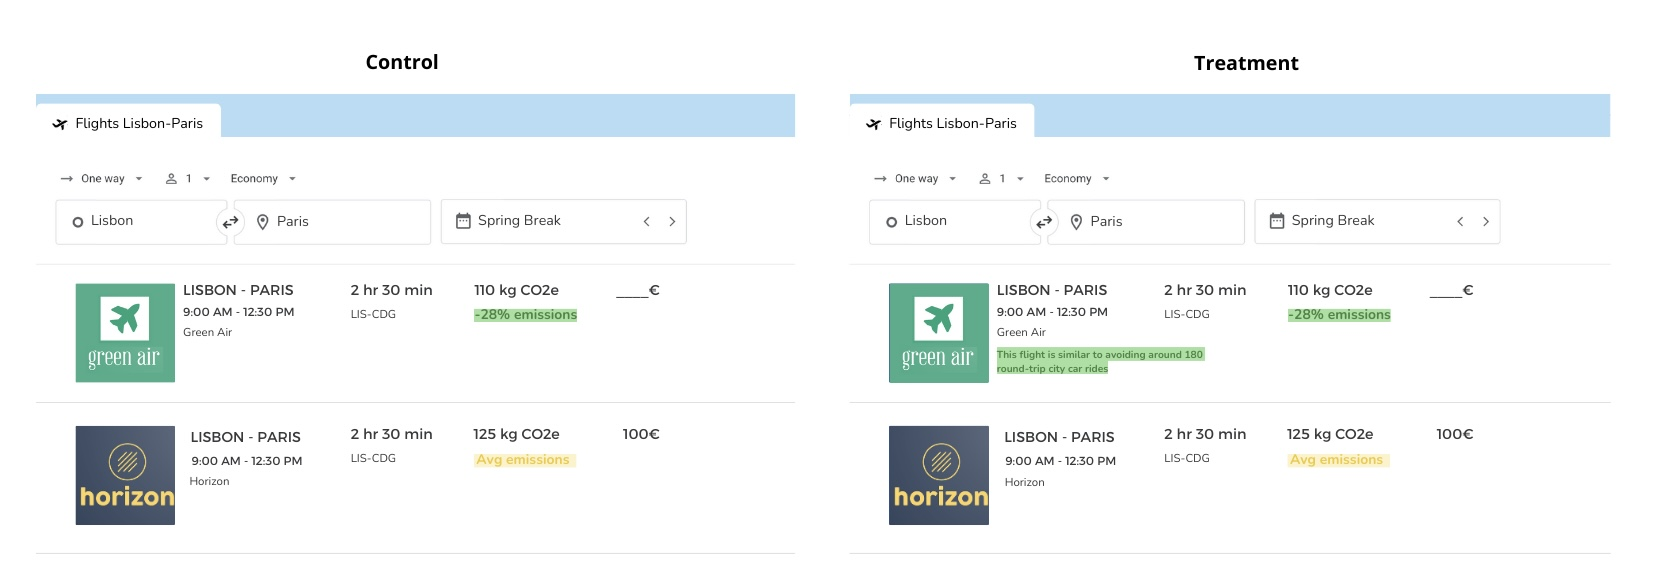
\includegraphics{ControlvsTreat.jpg}
\caption{Images displayed for Control and Treatment Groups in Survey}
\end{figure}

From an ethical standpoint, we prioritized participant confidentiality
and voluntary participation. A confidentiality statement was included at
the beginning of the survey, informing participants that their responses
would remain anonymous, data would be kept confidential, and
participation was entirely voluntary.

The complete survey design and materials can be found in the appendix.

To rigorously evaluate the causal effect of framing on WTP, we specify
the following baseline regression model:

\[
WTP_{i} = \beta_0 + \beta_1 \text{Humanized}_{i} + \epsilon_{i}
\]

Where \(\text{WTP}_{i}\) represents the willingness to pay for
individual \(\text{i}\) and \(\text{Humanized}_{i}\) is a binary
variable indicating whether the participant received the humanized
framing. The coefficient \(\beta_1\) captures the direct impact of
framing on WTP.

Since treatment effects may vary across individuals, we extend the model
to account for heterogeneous treatment effects by incorporating key
demographic covariates :

\[
WTP_{i} = \beta_0 + \beta_1 \text{Humanized}_{i} + \beta_2 \text{Gender}_{i} + \beta_3 \text{Age}_{i} + \beta_4 \text{Income}_{i} + \beta_4 \text{Nationality}_{i} + \epsilon_{i}
\]

By including these additional covariates, we control for potential
confounding factors and explore whether certain subgroups (e.g.,
frequent travelers) exhibit stronger responses to the treatment. This
approach allows us to better understand the mechanisms through which
framing influences WTP.

To determine the appropriate sample size for detecting a meaningful
effect, we conducted a power analysis for a one-sided two-sample t-test.
Given a small effect size (d = 0.2), a significance level of \(\alpha\)
= 0.05, and a power of 0.8, the required sample size was calculated
using the \texttt{power.t.test} function in R. The analysis indicated
that the sample should contain approximately 256 participants to ensure
the desired statistical power to detect the expected effect.

\begin{table}[!htbp] \centering 
  \caption{Sample Size} 
  \label{tab:ate} 
\begin{tabular}{@{\extracolsep{5pt}} cc} 
\\[-1.8ex]\hline 
\hline \\[-1.8ex] 
Group & Results \\ 
\hline \\[-1.8ex] 
Estimated n & $256$ \\ 
Delta & $0.220$ \\ 
Significance Level & $0.050$ \\ 
Power & $0.800$ \\ 
True n & $258$ \\ 
\hline \\[-1.8ex] 
\end{tabular} 
\end{table}

\hypertarget{analysis-and-results}{%
\section{3. Analysis and Results}\label{analysis-and-results}}

To better understand the sample data, the following section provides a
comprehensive analysis of the characteristics and distributions of the
collected variables.

\hypertarget{data-description}{%
\subsection{3.1. Data Description}\label{data-description}}

The survey, conducted between March 16 and March 22, 2025, yielded 208
usable responses. We also considered 50 more entries from Varteo's
synthetic survey, reaching the final size of 258 responses; while 258
responses provide a reasonable basis for statistical analysis, the
sample may still be considered moderate rather than large, which could
limit the robustness of subgroup analyses. A larger sample would
increase statistical power and allow for more precise estimation of
treatment effects.

To ensure a clean and structured dataset for analysis, we first loaded
the survey data and removed unnecessary rows and columns, including
automatically generated metadata from Qualtrics. We then filtered out
incomplete responses and those from preview distributions to maintain
data integrity. Next, we renamed variables for consistency and ease of
use in R. A treatment group variable was created based on the
`ImageShown' column, classifying participants accordingly. We proceeded
by converting categorical variables related to environmental and ethical
attitudes into numerical scales, facilitating quantitative analysis. To
enhance interpretability, we computed mean scores for environmental and
ethical perceptions, aggregating responses across multiple related
survey items. These preprocessing steps ensured that our dataset was
well-structured, reliable, and ready for statistical analysis.

\begin{table}[!htbp] \centering 
  \caption{Overview and Description of Variables} 
  \label{} 
\begin{tabular}{@{\extracolsep{5pt}} cccc} 
\\[-1.8ex]\hline 
\hline \\[-1.8ex] 
Variable & Description & Format & Collection \\ 
\hline \\[-1.8ex] 
flight\_frequency & Flight frequency of the participant & Factor & Drop-down menu \\ 
nationality & Nationality of the participant & Factor & Drop-down menu \\ 
gender & Gender of the participant & Factor & Drop-down menu \\ 
age & Binned age of the participant & Factor & Drop-down menu \\ 
work\_status & Profession of the participant & Factor & Drop-down menu \\ 
education\_level & Education level of the participant & Factor & Drop-down menu \\ 
household\_income & Household income level of the participant & Factor & Drop-down menu \\ 
group & Indicating assigned treatment or control group & Factor & Automatically \\ 
env\_mean & Environmental mean score of the participant & Numeric & 5-point scale \\ 
eth\_mean & Ethical mean score of the participant & Numeric & 5-point scale \\ 
wtp & Willingness to pay & Numeric & Slider \\ 
\hline \\[-1.8ex] 
\end{tabular} 
\end{table}

Our primary outcome variable was WTP, which measured participants'
willingness to pay for a lower-emission flight under different treatment
or control conditions. Participants provided their responses via a
slider input, allowing for precise and unrestricted values. Given the
potential influence of environmental and ethical attitudes on
willingness to pay, we computed mean scores for both constructs using a
5-point Likert scale. The flight frequency of each participant was
recorded to assess their typical travel behavior. Demographic variables
such as nationality, gender, age, work status, education level, and
household income were collected using drop-down menus to ensure
consistency in responses. Lastly, participants were randomly assigned to
either the control or treatment group, which was recorded in the group
variable for experimental analysis.

The boxplot in Graph 1 below compares the Willingness to Pay (WTP) in
EUR between data collected through traditional Survey Data and Synthetic
Data generated via Varteo, across two groups: Control and Treatment.
Varteo employs a sophisticated algorithm that ensures synthetic personas
make decisions consistent with real individuals by continuously
monitoring their decision-making processes against real-world data. If a
synthetic persona deviates significantly from human behavior, it is
flagged for review to maintain the model's accuracy.

From the graph, we observe that the Survey Data and Synthetic Data
exhibit similar median WTP values across both Control and Treatment
groups. However, the Synthetic Data shows a slightly more compressed
distribution, suggesting that Varteo's modeling process reduces extreme
variations compared to Survey Data. The Survey Data displays a wider
interquartile range (IQR) and more pronounced outliers, particularly in
the higher WTP values. This indicates that responses from real
individuals may be more variable and prone to extreme valuations,
whereas Varteo's personas produce more stabilized predictions.

The comparison between synthetic and survey data in Appendix A reveals
some differences across key covariates. The synthetic data has a lower
proportion of respondents aged 18-24 (12\% vs.~39\%) and fewer females
(48\% vs.~60\%) compared to the survey data. Additionally, the
proportion of individuals with a bachelor's degree is higher in the
synthetic data (76\% vs.~43\%), as is the proportion of employed
respondents (82\% vs.~56\%) and Portuguese nationals (98\% vs.~82\%).
Importantly, Willingness to Pay (WTP) is lower in the synthetic data
(9.56 EUR vs.~12.87 EUR).

Considering these results, the following analysis will integrate
Varteo's data as a complementary source for real survey data, ensuring
robustness while maintaining real-world variability.

\includegraphics{Group_H_v8_files/figure-latex/plot1-1.pdf}

It is important to mention that concerns related to non-compliance,
attrition, and interference were minimal. Non-compliance was not an
issue since treatment assignment closely aligned with treatment receipt,
ensuring that all participants followed their assigned conditions.
Attrition was also not a major concern, as outcome data was collected
for nearly all respondents, minimizing the risk of bias due to missing
observations. Finally, interference was unlikely because participants
completed the survey independently, without exposure to or influence
from others' treatment assignments. These factors help ensure that the
estimated effects accurately reflect the intended causal relationships.

\hypertarget{exploratory-data-analysis}{%
\subsection{3.2. Exploratory Data
Analysis}\label{exploratory-data-analysis}}

\hypertarget{outcome-variable---willingness-to-pay}{%
\subsubsection{Outcome Variable - Willingness to
Pay}\label{outcome-variable---willingness-to-pay}}

To begin our Exploratory Data Analysis, we first examine how our outcome
variable is distributed across groups.

The histogram below shows the distribution of Willingness to Pay (in €).
In both groups, the most common values chosen were 0 and 20€. While the
majority of participants selected price points between 0 and 20€, the
treatment group showed a slight preference for price points between 20
and 40€. Notably, the distribution is not bell-shaped, indicating that a
non-parametric test may be more appropriate for further analysis.

\includegraphics{Group_H_v8_files/figure-latex/plot2-1.pdf}

\hypertarget{main-covariates}{%
\subsubsection{Main Covariates}\label{main-covariates}}

While examining the distribution of our outcome variable (WTP) provides
insights into its overall behavior, it is equally important to explore
the distribution of key covariates. These variables may influence WTP
and help us understand whether differences across groups arise from the
treatment itself or pre-existing characteristics.

As can be seen from the far left graph below, approximately one third of
the participants are aged between 18-24 (n = 87). There are
significantly more female participants than male (n = 148 vs n = 105).
Most of the participants were of Portuguese nationality (n = 219),
followed by German (n = 19). Other different nationalities were found to
be in the minority and were grouped together for visualization purposes
(n = 20).

\includegraphics{Group_H_v8_files/figure-latex/plot3-1.pdf} The survey
also gathered data on participants' education levels, revealing that the
majority held a Bachelor's degree (n = 128), followed by those with a
Master's degree (n = 68). A smaller portion of respondents had a
Doctor's degree (n = 1). Regarding employment status, the sample was
largely composed of full-time workers (n = 158) and students (n = 72).

\includegraphics{Group_H_v8_files/figure-latex/plot4-1.pdf}

Graph 9 reveals an interesting trend: individuals who exhibit higher
levels of environmental concern, as measured through a series of survey
questions assessing their attitudes toward environmental issues, tend to
have a greater willingness to pay (WTP). This suggests a positive
relationship between environmental awareness and financial commitment to
environmentally friendly initiatives.

While this trend aligns with expectations, it is important to assess
whether this relationship holds when controlling for other factors. In
the next section, we further explore the role of covariates and
treatment effects through regression analysis to determine whether
environmental concern remains a significant predictor of WTP.

\begin{center}\includegraphics{Group_H_v8_files/figure-latex/plot8-1} \end{center}

\begin{itemize}
\tightlist
\item
  \textbf{Balance Check}
\end{itemize}

The likelihood ratio test below compares two models to assess whether
adding predictors improves model fit. Model 1 includes only an
intercept, while Model 2 includes age, nationality, education level,
gender, work status, and household income as predictors. The test yields
a chi-square statistic of 38.671 with 22 degrees of freedom and a
p-value of 0.01539, indicating a significant difference between the
models. In the context of a balance check, this suggests that these
covariates are not evenly distributed across groups --- if they were,
adding them would not significantly improve the model. The significant
result implies potential imbalance, meaning these factors might
systematically differ between groups.

The logistic regression analysis suggests that household income
significantly predicts treatment assignment, with higher-income
participants being more likely to be in the treatment group.
Additionally, the covariate balance table, (Appendix A), highlights
significant differences in nationality (p = 0.038) and work status (p =
0.021), with Portuguese respondents and non-full-time workers being
overrepresented in the treatment group. Although other variables, such
as education level and gender, appear balanced, the observed imbalances
in nationality, work status, and income could introduce bias. To address
this, adjustments using regression models will be considered in
subsequent analyses to ensure robust causal inference.

\begin{table}[!htbp] \centering 
  \caption{Likelihood Ratio Test Results} 
  \label{tab:likelihood} 
\begin{tabular}{@{\extracolsep{5pt}} cccccc} 
\\[-1.8ex]\hline 
\hline \\[-1.8ex] 
 & \#Df & LogLik & Df & Chisq & Pr(\textgreater Chisq) \\ 
\hline \\[-1.8ex] 
1 & $1$ & $$-$177.893$ & $$ & $$ & $$ \\ 
2 & $23$ & $$-$158.557$ & $22$ & $38.671$ & $0.015$ \\ 
\hline \\[-1.8ex] 
\end{tabular} 
\end{table}

\begin{itemize}
\tightlist
\item
  \textbf{Correlation Matrix}
\end{itemize}

Before proceeding with our regression models and subsequent tests, we
first decided we should examine the correlation between our variables
and willingness to pay (WTP).

The correlations are generally low, with all absolute values below 0.5.
This suggests that no single factor strongly drives WTP on its own.
However, the sign and significance of these correlations can still
provide meaningful insights.

Within the treatment group, there is a positive correlation between
environmental concern (env\_mean) and WTP, meaning individuals who care
more about environmental issues are willing to pay more. Conversely,
ethical concern (eth\_mean) shows no significant correlation with WTP.
This suggests that environmental concerns might have a stronger
influence on WTP than ethical values in the treatment group.

Age shows a negative correlation with WTP, especially in the 35-44 and
45-54 age groups; income does not appear to significantly affect WTP, as
the correlation is minimal across different income categories.
Similarly, flight frequency does not have a strong impact on WTP, with
only the 6-10 times a year category showing a slight negative
relationship, though not statistically significant.

Gender and other demographic factors were also analyzed. The
correlations between these factors and WTP are low, suggesting that
there are no clear patterns based solely on these characteristics.

\includegraphics{Group_H_v8_files/figure-latex/heatmaps-1.pdf}

\hypertarget{ate-and-mean-comparison}{%
\subsubsection{ATE and Mean Comparison}\label{ate-and-mean-comparison}}

While the correlation matrix provides insights into how different
variables relate to WTP, it does not establish causality. To further
investigate the effect of the treatment on WTP, we calculate the Average
Treatment Effect (ATE) and compare the mean WTP between treatment and
control groups. This allows us to assess whether any observed
differences in WTP can be attributed to the intervention rather than
underlying correlations.

Graph 8 below compares the Willingness to Pay (WTP) between participants
in the Control and Treatment groups. The distributions are fairly
similar, with both groups having a median around 10€. Additionally, the
interquartile range (IQR) for both groups spans approximately 5€ to 20€,
indicating comparable variability in responses.

While there does not appear to be a notable difference in WTP between
groups, suggesting that the treatment effect may be small, we will
conduct formal statistical tests to determine whether this difference is
statistically significant.

To quantify the impact of framing on participants' willingness to pay,
we estimated the true Average Treatment Effect (ATE) across all
participants. The results, summarized in the table below, show the mean
WTP for each group:

\includegraphics{Group_H_v8_files/figure-latex/ate-1.pdf}

The ATE of 0.130 suggests that the treatment increased the average WTP
compared to the control group. This indicates that framing had a
positive impact, though the magnitude is relatively small. To determine
whether this difference is statistically significant or if it could have
arisen due to random chance, we will conduct formal statistical tests in
the following section.

\hypertarget{findings}{%
\subsection{3.3. Findings}\label{findings}}

Starting off our regression analysis, we feel it is important to first
assess whether there are baseline differences between the treatment and
control groups. Conducting a preliminary test, such as a Welch
Two-Sample t-test, helps determine if the groups are already
significantly different in terms of their willingness to pay (WTP)
before accounting for additional covariates. If a significant difference
were found, it would suggest that factors other than the treatment
itself might be influencing WTP, highlighting the need for careful
adjustment in the regression model. Conversely, if no significant
difference is found, it provides reassurance that any potential effects
observed in the regression analysis are more likely to be attributable
to the included explanatory variables rather than pre-existing
imbalances.

The table below we have the results of the Welch Two-Sample t-test,
which indicate that there is no significant difference in the mean
willingness to pay (WTP) between the control group (M = 12.16) and the
treatment group (M = 12.29), t(250.77) = -0.09, p = 0.9287. The p-value
is much higher than the conventional significance threshold of 0.05,
suggesting that any observed difference is likely due to random
variation rather than a true effect.

The 95\% confidence interval (-3.26, 3.02) includes zero, further
supporting the conclusion that the two groups do not significantly
differ in their WTP for lower-emission flights. Therefore, we fail to
reject the null hypothesis, indicating that the treatment did not have a
measurable impact on WTP.

\begin{table}[!htbp] \centering 
  \caption{Welch Two-Sample t-test Results} 
  \label{} 
\begin{tabular}{@{\extracolsep{5pt}} ccc} 
\\[-1.8ex]\hline 
\hline \\[-1.8ex] 
 & Statistic & Value \\ 
\hline \\[-1.8ex] 
1 & t-value & $$-$0.090$ \\ 
2 & df & $250.775$ \\ 
3 & p-value & $0.929$ \\ 
4 & 95\% CI Lower & $$-$2.867$ \\ 
5 & 95\% CI Upper & $2.618$ \\ 
6 & Mean (Control) & $12.161$ \\ 
7 & Mean (Treatment) & $12.286$ \\ 
\hline \\[-1.8ex] 
\end{tabular} 
\end{table}

After confirming that there was no significant difference in WTP between
the control and treatment groups with the Welch t-test, we wanted to
ensure that this test was indeed appropriate. Although the t-test is
generally preferred because it compares means rather than distributions
(as the Mann-Whitney U test does), it relies on the assumption of
normally distributed data. Since we believe our sample size is
statistically large enough for the Central Limit Theorem (CLT) to hold,
this assumption may not be critical. However, to avoid potential biases
and strengthen our conclusions, we decided to formally test for
normality.

The results of the Shapiro-Wilk test indicate that the assumption of
normality is violated for both the control (W = 0.897, p \textless{}
0.001) and treatment (W = 0.888, p \textless{} 0.001) groups. Since the
p-values are significantly below 0.05, we reject the null hypothesis of
normality, suggesting that the distribution of WTP (Willingness to Pay)
is not normally distributed in either group.

\begin{table}[!htbp] \centering 
  \caption{Shapiro-Wilk Test Results} 
  \label{} 
\begin{tabular}{@{\extracolsep{5pt}} cccc} 
\\[-1.8ex]\hline 
\hline \\[-1.8ex] 
 & Group & W & p\_value \\ 
\hline \\[-1.8ex] 
1 & Control & $0.897$ & 1.67190e-07 \\ 
2 & Treatment & $0.888$ & 7.14342e-09 \\ 
\hline \\[-1.8ex] 
\end{tabular} 
\end{table}

Given this result, we could still justify using the t-test under the
assumption that our sample size is sufficiently large for the CLT to
apply. However, to ensure robustness, we performed an additional
non-parametric test (Mann-Whitney U test), which does not assume
normality. The resulting p-value (0.9785) is considerably high (greater
than 0.05), indicating that we fail to reject the null hypothesis. This
suggests strong evidence that the distribution of WTP is statistically
similar between the groups, implying that the treatment had no
significant effect on participants' willingness to pay.

Since both tests led to the same conclusion---that the treatment had no
effect on WTP---we can confidently assert that our findings are not
driven by assumptions about normality and that the treatment did not
have a measurable impact on WTP.

\begin{table}[!htbp] \centering 
  \caption{Mann-Whitney U Test Results} 
  \label{tab:mannwhitney} 
\begin{tabular}{@{\extracolsep{5pt}} cc} 
\\[-1.8ex]\hline 
\hline \\[-1.8ex] 
Statistic & P\_Value \\ 
\hline \\[-1.8ex] 
$8,276.5000$ & $0.9785$ \\ 
\hline \\[-1.8ex] 
\end{tabular} 
\end{table}

Although our previous tests indicated that the treatment likely had no
effect on WTP, we decided to further explore this relationship by
controlling for additional covariates. By doing so, we aimed to
determine whether any underlying factors influenced WTP and to confirm
that the treatment remained statistically insignificant even when
accounting for these variables. To achieve this, we implemented a
baseline model (including only treatment) and an expanded model
incorporating covariates and interaction effects.

We conducted an Ordinary Least Squares (OLS) regression analysis to
assess the relationship between the treatment and other independent
variables with WTP. The regression model helps identify the impact of
each factor while accounting for the influence of others. We considered
several different models with varying sets of covariates.

The baseline model serves as the baseline, including only the treatment
variable (group). The coefficient for group (\(\beta\) = 0.125) is small
and statistically insignificant, indicating that the treatment had no
observable impact on WTP. The R² value is nearly zero, meaning that the
model explains virtually none of the variation in WTP. This suggests
that simply receiving the treatment is not enough to predict changes in
WTP.

The extended model further expands the analysis by adding nationality
and interaction effects. A notable new finding is that Portuguese
participants exhibit significantly lower WTP (\(\beta\) = -8.970, p
\textless{} 0.05), suggesting that nationality plays a crucial role in
willingness to pay.

The R² for the extended model improves to 0.239, meaning that 23.9\% of
the variance in WTP is explained by the included covariates. However,
the treatment variable (group) remains statistically insignificant,
reinforcing the conclusion that the intervention did not meaningfully
influence participants' WTP.

Models 1 and 4 are displayed in the table below, while the other
evaluated models can be found in Appendix A.

\begin{table}[!htbp] \centering 
  \caption{Regression Results for WTP Models} 
  \label{} 
\small 
\begin{tabular}{@{\extracolsep{3pt}}lcc} 
\\[-1.8ex]\hline 
\hline \\[-1.8ex] 
 & \multicolumn{2}{c}{\textit{Dependent variable:}} \\ 
\cline{2-3} 
\\[-1.8ex] & \multicolumn{2}{c}{WTP} \\ 
 & Baseline Model & Extended Model \\ 
\\[-1.8ex] & (1) & (2)\\ 
\hline \\[-1.8ex] 
 group & 0.125 (1.398) & 0.953 (1.437) \\ 
  flight\_frequency6-10 times a year &  & $-$4.789$^{*}$ (2.902) \\ 
  flight\_frequencyMore than 10 times a year &  & $-$0.015 (3.670) \\ 
  flight\_frequencyNever &  & 3.197 (2.670) \\ 
  flight\_frequencyOnce a year or less &  & 1.475 (1.664) \\ 
  household\_income1500 euros to 4999 euros per month &  & $-$0.038 (6.123) \\ 
  household\_income5000 euros to 7999 euros per month &  & $-$2.137 (6.274) \\ 
  household\_income8000 to 11999 euros per month &  & $-$2.706 (6.982) \\ 
  household\_incomeLess than 1500 euros per month &  & $-$3.898 (6.354) \\ 
  env\_mean &  & 3.724$^{***}$ (1.326) \\ 
  eth\_mean &  & 2.786 (2.038) \\ 
  age25-34 &  & $-$3.433 (2.412) \\ 
  age35-44 &  & $-$0.888 (3.345) \\ 
  age45-54 &  & $-$7.431$^{***}$ (2.653) \\ 
  age55-64 &  & $-$1.726 (3.221) \\ 
  age65+ &  & $-$5.336 (8.433) \\ 
  genderMale &  & 1.213 (1.435) \\ 
  genderNon-binary &  & 2.472 (28.968) \\ 
  genderPrefer not to say &  & 0.053 (5.145) \\ 
  nationalityOther: &  & $-$5.756 (4.059) \\ 
  nationalityPortugal &  & $-$8.970$^{**}$ (3.655) \\ 
  work\_statusPart-time worker/Intern &  & 1.183 (2.961) \\ 
  work\_statusRetired &  & 6.261 (10.688) \\ 
  work\_statusStudent &  & $-$1.529 (2.109) \\ 
  work\_statusUnemployed/Housewife &  & $-$2.546 (8.851) \\ 
  Constant & 12.161$^{***}$ (1.017) & $-$3.101 (8.274) \\ 
 \hline \\[-1.8ex] 
Observations & 258 & 255 \\ 
R$^{2}$ & 0.00003 & 0.239 \\ 
Adjusted R$^{2}$ & $-$0.004 & 0.156 \\ 
F Statistic & 0.008 (df = 1; 256) & 2.883$^{***}$ (df = 25; 229) \\ 
\hline 
\hline \\[-1.8ex] 
\textit{Note:}  & \multicolumn{2}{r}{$^{*}$p$<$0.1; $^{**}$p$<$0.05; $^{***}$p$<$0.01} \\ 
\end{tabular} 
\end{table}

\newpage

\hypertarget{discussion}{%
\section{4. Discussion}\label{discussion}}

\hypertarget{final-considerations}{%
\subsection{4.1. Final Considerations}\label{final-considerations}}

Internally, the study benefits from a completely randomized experimental
design, which enhances causal inference by reducing systematic
differences between the treatment and control groups. The inclusion of
synthetic data from Varteo also contributes to the robustness of the
findings by offering a supplementary dataset that closely mirrors
real-world decision-making patterns.

Externally, while the sample includes participants from diverse
geographical backgrounds, it is still skewed toward Portuguese
respondents, potentially limiting the generalizability of the findings.
Additionally, the survey setting differs from real-world flight booking
scenarios, where consumers face additional constraints, such as time
pressure and brand preferences.

The results show that the humanized framing of carbon emissions did not
significantly increase willingness to pay (WTP) for lower-emission
flights. While this does not negate the psychological impact of framing,
it suggests that WTP might be driven more by personal values and
economic considerations than by information presentation alone.

Another important factor at play was that the assumption of normality
was violated in both treatment and control groups, as indicated by the
Shapiro-Wilk test. This necessitated the use of non-parametric tests,
which may have reduced the power of the statistical analysis.

Some additional limitations of this study should be acknowledged. First,
the sample is not fully representative of the global traveling
population, as Portuguese participants constitute a large majority. This
demographic imbalance may introduce cultural biases that affect the
generalizability of the findings, particularly regarding attitudes
toward sustainability and willingness to pay (WTP) for lower-emission
flights.

Second, the reliance on self-reported data presents inherent challenges.
Respondents may overestimate or underestimate their WTP due to the
absence of real financial stakes in the decision-making process.
Hypothetical bias remains a concern, as individuals might express a
willingness to pay more for greener options in a survey setting but
behave differently in real-world purchase scenarios.

Finally, the experimental treatment was administered in a one-time
survey, whereas real consumer behavior is often shaped by repeated
exposure to sustainability messaging over time. In practice, travelers
may develop stronger or weaker preferences for lower-emission flights
through cumulative interactions with environmental campaigns, airline
policies, or social influences.

\hypertarget{summary-and-recommendations}{%
\subsection{4.2. Summary and
Recommendations}\label{summary-and-recommendations}}

The results indicate that the humanized framing of carbon emissions did
not produce a statistically significant increase in willingness to pay
(WTP) for lower-emission flights. The mean WTP difference between the
treatment and control groups was negligible, and the regression results
confirm the absence of a significant effect (p \textgreater{} 0.05).
This suggests that, while framing may influence consumer perceptions, it
does not necessarily translate into higher financial commitments toward
sustainable travel.

A statistically significant relationship was observed between
environmental concern scores and WTP, independent of the framing
condition. Individuals with higher self-reported environmental concern
exhibited a greater willingness to pay for greener flights, reinforcing
the idea that pre-existing environmental values play a stronger role in
decision-making than subtle variations in information presentation.

Frequent flyers (6--10 trips per year) demonstrated a lower WTP for
sustainable flight options compared to infrequent travelers. Regression
analysis confirms a statistically significant negative effect. This may
be attributed to cost sensitivity or established habitual behaviors,
which make price a dominant factor in their decision-making.

While broad demographic variables such as income and education did not
exhibit statistically significant direct effects on WTP, Portuguese
participants showed a notably lower WTP relative to other nationalities.
This finding highlights potential cultural influences that shape
attitudes toward sustainable travel and suggests that country-specific
factors, such as environmental policies and economic conditions, may
mediate consumer behavior.

To better understand how framing affects behavior, future studies should
test these effects in actual booking environments where real financial
commitments are made. Examining how repeated exposure to sustainability
messaging affects WTP over time could also provide more insights into
the long-term impact of framing.

Exploring different types of humanized framing could be a potential
source of new findings, such as social norm messaging (e.g., ``80\% of
travelers choose greener flights'') or financial incentives tied to
emissions reduction. Given the observed differences in WTP based on
nationality, further studies should investigate how cultural norms and
economic conditions influence sustainable travel decisions.

Overall, while this study does not find strong evidence that humanized
framing alone significantly increases WTP, it provides valuable insights
into the factors that drive sustainable travel decisions. These findings
can inform more effective strategies for promoting eco-friendly travel
choices in the aviation industry.

\hypertarget{ai-disclaimer}{%
\section{5. AI Disclaimer}\label{ai-disclaimer}}

AI was used for the creation of this report in a limited scope. The main
use case of ChatGPT was the debugging of code. Furthermore, minor
paragraphs were rephrased.

\newpage

\hypertarget{bibliography}{%
\section{Bibliography}\label{bibliography}}

Baumeister, C., Carroll, B., Crosby, M., Thompson, L., \& Best, J.
(2022). Consumer preferences for sustainable air travel: Evidence from
discrete choice experiments. Journal of Sustainable Travel Research,
18(3), 245-267.

Bergero, L., Smith, A., \& Huang, Y. (2023). Decarbonizing aviation:
Challenges and opportunities for net-zero emissions. Energy \&
Environmental Policy, 29(1), 56-78.

Carroll, B., Johnson, R., \& Lee, D. (2022). Understanding the impact of
emissions transparency on airline passenger behavior. Transportation
Economics Review, 35(4), 512-534.

Crosby, M., Thompson, L., \& Best, J. (2024). The role of price and
emissions data in flight selection: A behavioral approach. Journal of
Consumer Research, 51(2), 199-221.

Gössling, S., Hanna, P., Higham, J., Cohen, S. A., \& Hopkins, D.
(2021). Can we fly less? Evaluating the potential of behavioral change
strategies for reducing air travel demand. Journal of Air Transport
Management, 91, 101973.

Johnson, R., \& Lee, D. (2020). Framing environmental information to
influence consumer decision-making. Journal of Behavioral Economics \&
Policy, 12(2), 87-103.

Lee, D. S., Fahey, D. W., Skowron, A., Allen, M. R., Burkhardt, U.,
Chen, Q., \ldots{} \& Wilcox, L. J. (2021). The contribution of global
aviation to anthropogenic climate forcing for 2000--2018. Atmospheric
Environment, 244, 117834.

Lee, D. S., Pitari, G., Grewe, V., Gierens, K., Penner, J. E., Petzold,
A., \ldots{} \& Berntsen, T. (2009). Aviation and global climate change
in the 21st century. Atmospheric Environment, 43(22-23), 3520-3537.

Sanguinetti, A., \& Amenta, P. (2022). The psychology of eco-friendly
travel decisions: Willingness to pay for sustainable aviation.
Environmental Psychology Review, 14(1), 34-49.

Smith, J., Taylor, M., \& Green, P. (2021). Humanizing climate data: How
framing impacts consumer perception of carbon emissions. Journal of
Environmental Communication, 25(2), 147-163.

Song, H., Liu, X., \& Wang, J. (2024). Emissions labeling and consumer
behavior: Evidence from airline booking platforms. Journal of
Sustainable Aviation, 11(3), 301-317.

Travalyst. (2024). Sustainable travel insights: The impact of emissions
transparency on consumer behavior. Retrieved from www.travalyst.org.

\newpage

\hypertarget{appendix-a}{%
\section{Appendix A}\label{appendix-a}}

\begin{table}[!htbp] \centering 
  \caption{Comparison of Covariates Between Synthetic and Survey Data} 
  \label{} 
\begin{tabular}{@{\extracolsep{5pt}} ccc} 
\\[-1.8ex]\hline 
\hline \\[-1.8ex] 
Covariate & Survey Data & Synthetic Data \\ 
\hline \\[-1.8ex] 
DistributionChannel & Survey Data & Synthetic Data \\ 
Age\_18\_24 & 0.39 & 0.12 \\ 
Gender\_Female & 0.60 & 0.48 \\ 
Educ\_Bachelor & 0.43 & 0.76 \\ 
Work\_Employed & 0.56 & 0.82 \\ 
Nat\_Portugal & 0.82 & 0.98 \\ 
WTP & 12.87 &  9.56 \\ 
\hline \\[-1.8ex] 
\end{tabular} 
\end{table}

\begin{table}[!htbp] \centering 
  \caption{Proportion of Key Covariates by Group in Synthetic and Survey Data} 
  \label{} 
\begin{tabular}{@{\extracolsep{5pt}} ccc} 
\\[-1.8ex]\hline 
\hline \\[-1.8ex] 
Covariate & Control & Treatment \\ 
\hline \\[-1.8ex] 
group & $0$ & $1$ \\ 
Age\_18\_24\_Survey Data & $0.270$ & $0.490$ \\ 
Age\_18\_24\_Synthetic Data & $0.170$ & $0.080$ \\ 
Gender\_Female\_Survey Data & $0.630$ & $0.570$ \\ 
Gender\_Female\_Synthetic Data & $0.460$ & $0.500$ \\ 
Educ\_Bachelor\_Survey Data & $0.450$ & $0.420$ \\ 
Educ\_Bachelor\_Synthetic Data & $0.750$ & $0.770$ \\ 
Work\_Employed\_Survey Data & $0.680$ & $0.460$ \\ 
Work\_Employed\_Synthetic Data & $0.790$ & $0.850$ \\ 
Nat\_Portugal\_Survey Data & $0.740$ & $0.880$ \\ 
Nat\_Portugal\_Synthetic Data & $0.960$ & $1$ \\ 
WTP\_Survey Data & $12.670$ & $13.040$ \\ 
WTP\_Synthetic Data & $10.170$ & $9$ \\ 
\hline \\[-1.8ex] 
\end{tabular} 
\end{table}

\begin{table}[!htbp] \centering 
  \caption{Covariates table: Balance check} 
  \label{} 
\begin{tabular}{@{\extracolsep{5pt}} cccccc} 
\\[-1.8ex]\hline 
\hline \\[-1.8ex] 
 & Characteristic & Category & Control & Treatment & p-value \\ 
\hline \\[-1.8ex] 
1 &  & age &  &  & NA \\ 
2 &  & 18-24 & 29 (33\%) & 58 (67\%) & NA \\ 
3 &  & 25-34 & 27 (44\%) & 34 (56\%) & NA \\ 
4 &  & 35-44 & 18 (69\%) & 8 (31\%) & NA \\ 
5 &  & 45-54 & 19 (45\%) & 23 (55\%) & NA \\ 
6 &  & 55-64 & 22 (63\%) & 13 (37\%) & NA \\ 
7 &  & 65+ & 3 (43\%) & 4 (57\%) & NA \\ 
8 & nationality & nationality &  &  & 0.0383 \\ 
9 &  & Germany & 13 (68\%) & 6 (32\%) & NA \\ 
10 &  & Other: & 12 (60\%) & 8 (40\%) & NA \\ 
11 &  & Portugal & 93 (42\%) & 126 (58\%) & NA \\ 
12 & education\_level & education\_level &  &  & 0.3488 \\ 
13 &  & Bachelor's or equivalent & 60 (47\%) & 68 (53\%) & NA \\ 
14 &  & College/University & 16 (47\%) & 18 (53\%) & NA \\ 
15 &  & Doctorate or equivalent & 1 (100\%) & 0 (0\%) & NA \\ 
16 &  & High School/Senior High & 8 (30\%) & 19 (70\%) & NA \\ 
17 &  & Masters or equivalent & 33 (49\%) & 35 (51\%) & NA \\ 
18 & gender & gender &  &  & 0.6056 \\ 
19 &  & Female & 70 (47\%) & 78 (53\%) & NA \\ 
20 &  & Male & 46 (44\%) & 59 (56\%) & NA \\ 
21 &  & Non-binary & 0 (0\%) & 2 (100\%) & NA \\ 
22 &  & Prefer not to say & 2 (67\%) & 1 (33\%) & NA \\ 
23 & work\_status & work\_status &  &  & 0.0214 \\ 
24 &  & Full time worker & 83 (53\%) & 75 (47\%) & NA \\ 
25 &  & Part-time worker/Intern & 9 (53\%) & 8 (47\%) & NA \\ 
26 &  & Retired & 1 (17\%) & 5 (83\%) & NA \\ 
27 &  & Student & 24 (33\%) & 48 (67\%) & NA \\ 
28 &  & Unemployed/Housewife & 1 (20\%) & 4 (80\%) & NA \\ 
29 & household\_income & household\_income &  &  & 0.329 \\ 
30 &  & 12000+ euros per month & 6 (86\%) & 1 (14\%) & NA \\ 
31 &  & 1500 euros to 4999 euros per month & 65 (45\%) & 81 (55\%) & NA \\ 
32 &  & 5000 euros to 7999 euros per month & 19 (46\%) & 22 (54\%) & NA \\ 
33 &  & 8000 to 11999 euros per month & 7 (41\%) & 10 (59\%) & NA \\ 
34 &  & Less than 1500 euros per month & 21 (45\%) & 26 (55\%) & NA \\ 
\hline \\[-1.8ex] 
\end{tabular} 
\end{table}

\begin{table}[!htbp] \centering 
  \caption{Other Regression Results for WTP Models} 
  \label{} 
\begin{tabular}{@{\extracolsep{5pt}}lcc} 
\\[-1.8ex]\hline 
\hline \\[-1.8ex] 
 & \multicolumn{2}{c}{\textit{Dependent variable:}} \\ 
\cline{2-3} 
\\[-1.8ex] & \multicolumn{2}{c}{Willingness to Pay (WTP)} \\ 
 & Model 2 & Model 3 \\ 
\\[-1.8ex] & (1) & (2)\\ 
\hline \\[-1.8ex] 
 group & 0.548 & 0.505 \\ 
  & (1.372) & (1.410) \\ 
  & & \\ 
 flight\_frequency6-10 times a year & $-$4.626$^{*}$ & $-$4.938$^{*}$ \\ 
  & (2.520) & (2.615) \\ 
  & & \\ 
 flight\_frequencyMore than 10 times a year & $-$0.956 & 0.920 \\ 
  & (3.495) & (3.345) \\ 
  & & \\ 
 flight\_frequencyNever & 2.201 & 2.597 \\ 
  & (2.408) & (2.516) \\ 
  & & \\ 
 flight\_frequencyOnce a year or less & 0.924 & 1.187 \\ 
  & (1.591) & (1.604) \\ 
  & & \\ 
 household\_income1500 euros to 4999 euros per month & $-$2.245 & $-$0.539 \\ 
  & (4.405) & (4.316) \\ 
  & & \\ 
 household\_income5000 euros to 7999 euros per month & $-$3.699 & $-$2.102 \\ 
  & (4.516) & (4.503) \\ 
  & & \\ 
 household\_income8000 to 11999 euros per month & $-$5.058 & $-$3.468 \\ 
  & (4.969) & (5.141) \\ 
  & & \\ 
 household\_incomeLess than 1500 euros per month & $-$4.989 & $-$3.809 \\ 
  & (4.542) & (4.438) \\ 
  & & \\ 
 env\_mean & 4.262$^{***}$ & 4.314$^{***}$ \\ 
  & (1.232) & (1.249) \\ 
  & & \\ 
 eth\_mean & 1.490 & 2.114 \\ 
  & (1.717) & (1.825) \\ 
  & & \\ 
 age25-34 &  & $-$0.610 \\ 
  &  & (1.772) \\ 
  & & \\ 
 age35-44 &  & 0.339 \\ 
  &  & (2.999) \\ 
  & & \\ 
 age45-54 &  & $-$6.478$^{***}$ \\ 
  &  & (1.909) \\ 
  & & \\ 
 age55-64 &  & 0.710 \\ 
  &  & (2.710) \\ 
  & & \\ 
 age65+ &  & 1.869 \\ 
  &  & (4.706) \\ 
  & & \\ 
 genderMale &  & 1.410 \\ 
  &  & (1.363) \\ 
  & & \\ 
 genderNon-binary &  & 2.761 \\ 
  &  & (7.809) \\ 
  & & \\ 
 genderPrefer not to say &  & 2.747 \\ 
  &  & (4.172) \\ 
  & & \\ 
 Constant & $-$7.788 & $-$11.859$^{**}$ \\ 
  & (5.659) & (5.728) \\ 
  & & \\ 
\hline \\[-1.8ex] 
Observations & 255 & 255 \\ 
R$^{2}$ & 0.143 & 0.195 \\ 
Adjusted R$^{2}$ & 0.104 & 0.130 \\ 
F Statistic & 3.685$^{***}$ (df = 11; 243) & 2.998$^{***}$ (df = 19; 235) \\ 
\hline 
\hline \\[-1.8ex] 
\textit{Note:}  & \multicolumn{2}{r}{$^{*}$p$<$0.1; $^{**}$p$<$0.05; $^{***}$p$<$0.01} \\ 
\end{tabular} 
\end{table}

\newpage

\hypertarget{appendix-b}{%
\section{Appendix B}\label{appendix-b}}

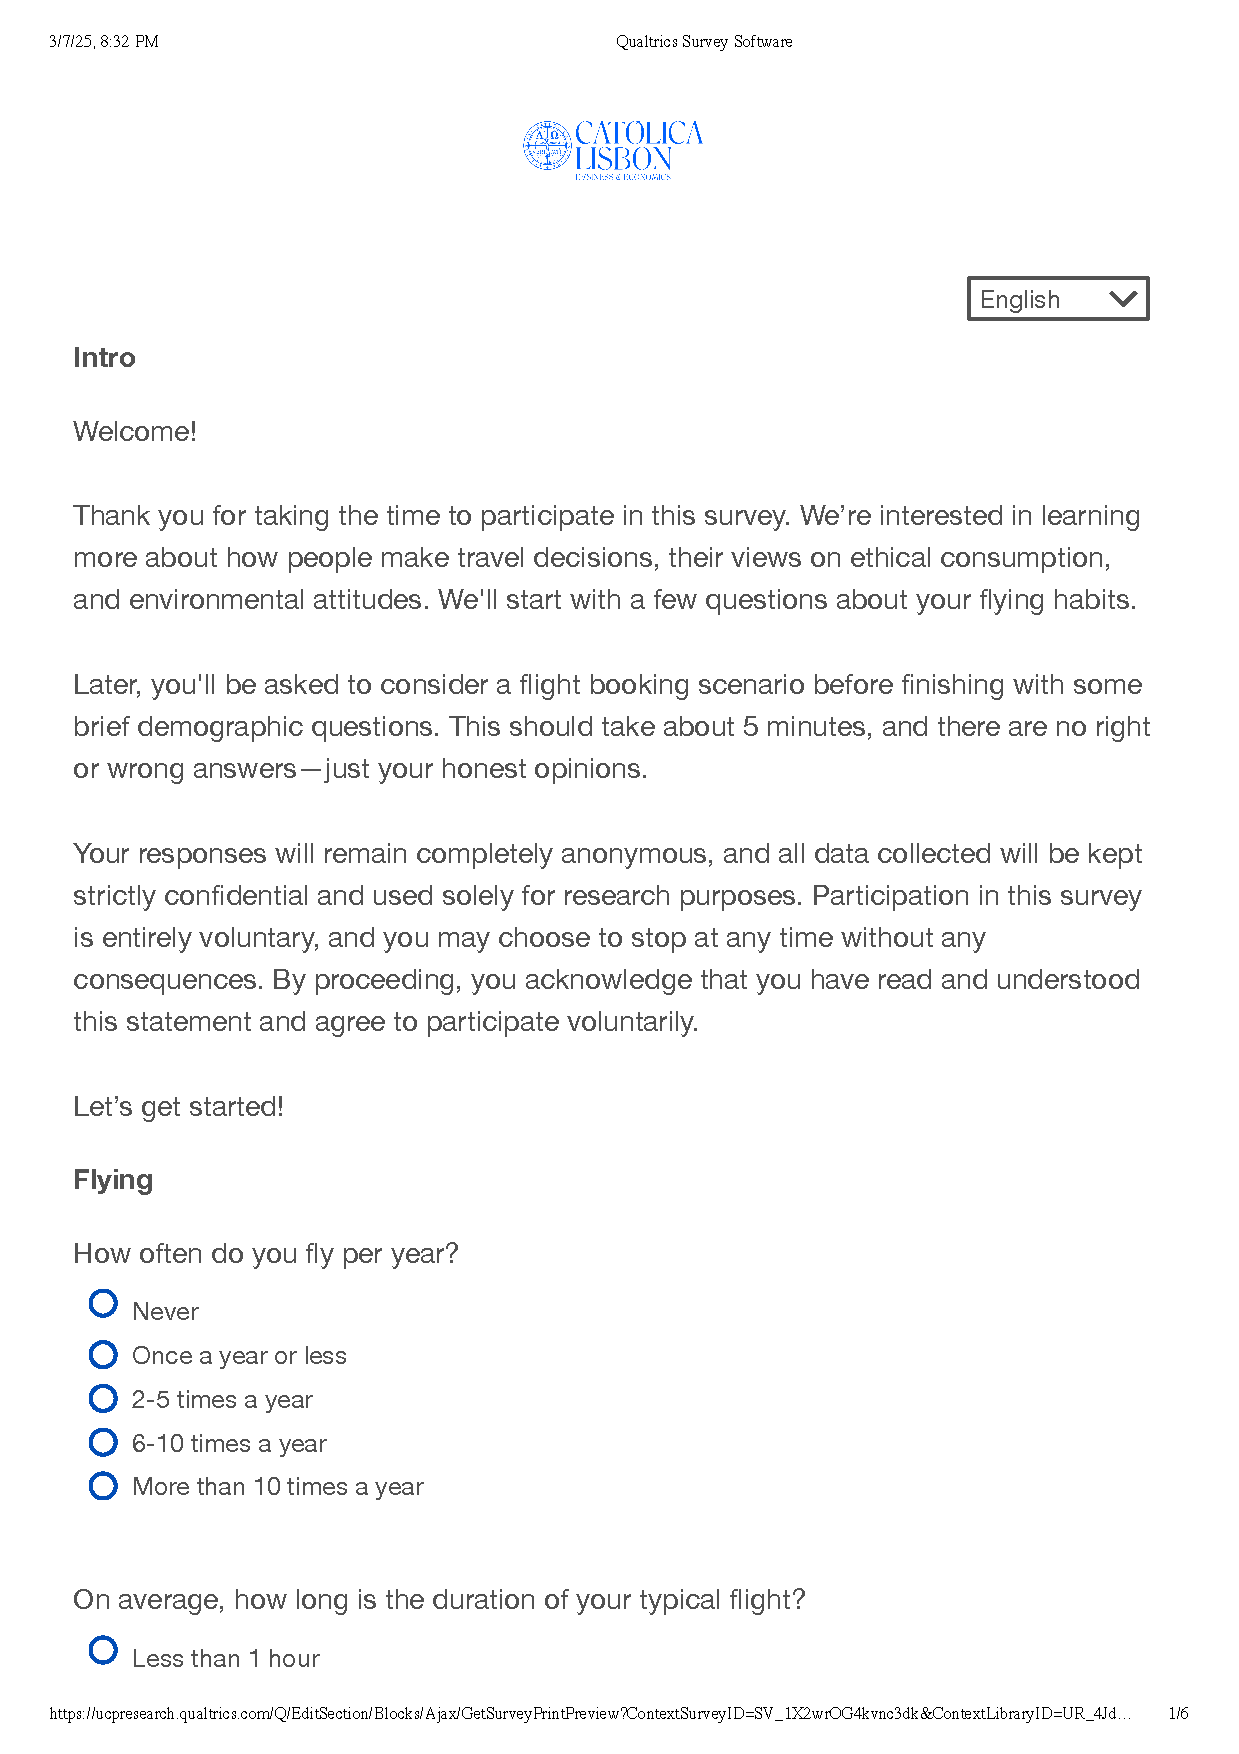
\includepdf[pages=-]{qualtrics_survey.pdf}

\end{document}
